% Options for packages loaded elsewhere
\PassOptionsToPackage{unicode}{hyperref}
\PassOptionsToPackage{hyphens}{url}
%
\documentclass[
]{article}
\usepackage{lmodern}
\usepackage{amssymb,amsmath}
\usepackage{ifxetex,ifluatex}
\ifnum 0\ifxetex 1\fi\ifluatex 1\fi=0 % if pdftex
  \usepackage[T1]{fontenc}
  \usepackage[utf8]{inputenc}
  \usepackage{textcomp} % provide euro and other symbols
\else % if luatex or xetex
  \usepackage{unicode-math}
  \defaultfontfeatures{Scale=MatchLowercase}
  \defaultfontfeatures[\rmfamily]{Ligatures=TeX,Scale=1}
\fi
% Use upquote if available, for straight quotes in verbatim environments
\IfFileExists{upquote.sty}{\usepackage{upquote}}{}
\IfFileExists{microtype.sty}{% use microtype if available
  \usepackage[]{microtype}
  \UseMicrotypeSet[protrusion]{basicmath} % disable protrusion for tt fonts
}{}
\makeatletter
\@ifundefined{KOMAClassName}{% if non-KOMA class
  \IfFileExists{parskip.sty}{%
    \usepackage{parskip}
  }{% else
    \setlength{\parindent}{0pt}
    \setlength{\parskip}{6pt plus 2pt minus 1pt}}
}{% if KOMA class
  \KOMAoptions{parskip=half}}
\makeatother
\usepackage{xcolor}
\IfFileExists{xurl.sty}{\usepackage{xurl}}{} % add URL line breaks if available
\IfFileExists{bookmark.sty}{\usepackage{bookmark}}{\usepackage{hyperref}}
\hypersetup{
  pdftitle={If you go down to the woods today\ldots.},
  pdfauthor={Matt Grainger},
  hidelinks,
  pdfcreator={LaTeX via pandoc}}
\urlstyle{same} % disable monospaced font for URLs
\usepackage[margin=1in]{geometry}
\usepackage{color}
\usepackage{fancyvrb}
\newcommand{\VerbBar}{|}
\newcommand{\VERB}{\Verb[commandchars=\\\{\}]}
\DefineVerbatimEnvironment{Highlighting}{Verbatim}{commandchars=\\\{\}}
% Add ',fontsize=\small' for more characters per line
\usepackage{framed}
\definecolor{shadecolor}{RGB}{248,248,248}
\newenvironment{Shaded}{\begin{snugshade}}{\end{snugshade}}
\newcommand{\AlertTok}[1]{\textcolor[rgb]{0.94,0.16,0.16}{#1}}
\newcommand{\AnnotationTok}[1]{\textcolor[rgb]{0.56,0.35,0.01}{\textbf{\textit{#1}}}}
\newcommand{\AttributeTok}[1]{\textcolor[rgb]{0.77,0.63,0.00}{#1}}
\newcommand{\BaseNTok}[1]{\textcolor[rgb]{0.00,0.00,0.81}{#1}}
\newcommand{\BuiltInTok}[1]{#1}
\newcommand{\CharTok}[1]{\textcolor[rgb]{0.31,0.60,0.02}{#1}}
\newcommand{\CommentTok}[1]{\textcolor[rgb]{0.56,0.35,0.01}{\textit{#1}}}
\newcommand{\CommentVarTok}[1]{\textcolor[rgb]{0.56,0.35,0.01}{\textbf{\textit{#1}}}}
\newcommand{\ConstantTok}[1]{\textcolor[rgb]{0.00,0.00,0.00}{#1}}
\newcommand{\ControlFlowTok}[1]{\textcolor[rgb]{0.13,0.29,0.53}{\textbf{#1}}}
\newcommand{\DataTypeTok}[1]{\textcolor[rgb]{0.13,0.29,0.53}{#1}}
\newcommand{\DecValTok}[1]{\textcolor[rgb]{0.00,0.00,0.81}{#1}}
\newcommand{\DocumentationTok}[1]{\textcolor[rgb]{0.56,0.35,0.01}{\textbf{\textit{#1}}}}
\newcommand{\ErrorTok}[1]{\textcolor[rgb]{0.64,0.00,0.00}{\textbf{#1}}}
\newcommand{\ExtensionTok}[1]{#1}
\newcommand{\FloatTok}[1]{\textcolor[rgb]{0.00,0.00,0.81}{#1}}
\newcommand{\FunctionTok}[1]{\textcolor[rgb]{0.00,0.00,0.00}{#1}}
\newcommand{\ImportTok}[1]{#1}
\newcommand{\InformationTok}[1]{\textcolor[rgb]{0.56,0.35,0.01}{\textbf{\textit{#1}}}}
\newcommand{\KeywordTok}[1]{\textcolor[rgb]{0.13,0.29,0.53}{\textbf{#1}}}
\newcommand{\NormalTok}[1]{#1}
\newcommand{\OperatorTok}[1]{\textcolor[rgb]{0.81,0.36,0.00}{\textbf{#1}}}
\newcommand{\OtherTok}[1]{\textcolor[rgb]{0.56,0.35,0.01}{#1}}
\newcommand{\PreprocessorTok}[1]{\textcolor[rgb]{0.56,0.35,0.01}{\textit{#1}}}
\newcommand{\RegionMarkerTok}[1]{#1}
\newcommand{\SpecialCharTok}[1]{\textcolor[rgb]{0.00,0.00,0.00}{#1}}
\newcommand{\SpecialStringTok}[1]{\textcolor[rgb]{0.31,0.60,0.02}{#1}}
\newcommand{\StringTok}[1]{\textcolor[rgb]{0.31,0.60,0.02}{#1}}
\newcommand{\VariableTok}[1]{\textcolor[rgb]{0.00,0.00,0.00}{#1}}
\newcommand{\VerbatimStringTok}[1]{\textcolor[rgb]{0.31,0.60,0.02}{#1}}
\newcommand{\WarningTok}[1]{\textcolor[rgb]{0.56,0.35,0.01}{\textbf{\textit{#1}}}}
\usepackage{graphicx,grffile}
\makeatletter
\def\maxwidth{\ifdim\Gin@nat@width>\linewidth\linewidth\else\Gin@nat@width\fi}
\def\maxheight{\ifdim\Gin@nat@height>\textheight\textheight\else\Gin@nat@height\fi}
\makeatother
% Scale images if necessary, so that they will not overflow the page
% margins by default, and it is still possible to overwrite the defaults
% using explicit options in \includegraphics[width, height, ...]{}
\setkeys{Gin}{width=\maxwidth,height=\maxheight,keepaspectratio}
% Set default figure placement to htbp
\makeatletter
\def\fps@figure{htbp}
\makeatother
\setlength{\emergencystretch}{3em} % prevent overfull lines
\providecommand{\tightlist}{%
  \setlength{\itemsep}{0pt}\setlength{\parskip}{0pt}}
\setcounter{secnumdepth}{-\maxdimen} % remove section numbering
<!--radix_placeholder_navigation_in_header-->
<meta name="distill:offset" content=""/>

<script type="application/javascript">

  window.headroom_prevent_pin = false;

  window.document.addEventListener("DOMContentLoaded", function (event) {

    // initialize headroom for banner
    var header = $('header').get(0);
    var headerHeight = header.offsetHeight;
    var headroom = new Headroom(header, {
      tolerance: 5,
      onPin : function() {
        if (window.headroom_prevent_pin) {
          window.headroom_prevent_pin = false;
          headroom.unpin();
        }
      }
    });
    headroom.init();
    if(window.location.hash)
      headroom.unpin();
    $(header).addClass('headroom--transition');

    // offset scroll location for banner on hash change
    // (see: https://github.com/WickyNilliams/headroom.js/issues/38)
    window.addEventListener("hashchange", function(event) {
      window.scrollTo(0, window.pageYOffset - (headerHeight + 25));
    });

    // responsive menu
    $('.distill-site-header').each(function(i, val) {
      var topnav = $(this);
      var toggle = topnav.find('.nav-toggle');
      toggle.on('click', function() {
        topnav.toggleClass('responsive');
      });
    });

    // nav dropdowns
    $('.nav-dropbtn').click(function(e) {
      $(this).next('.nav-dropdown-content').toggleClass('nav-dropdown-active');
      $(this).parent().siblings('.nav-dropdown')
         .children('.nav-dropdown-content').removeClass('nav-dropdown-active');
    });
    $("body").click(function(e){
      $('.nav-dropdown-content').removeClass('nav-dropdown-active');
    });
    $(".nav-dropdown").click(function(e){
      e.stopPropagation();
    });
  });
</script>

<style type="text/css">

/* Theme (user-documented overrideables for nav appearance) */

.distill-site-nav {
  color: rgba(255, 255, 255, 0.8);
  background-color: #0F2E3D;
  font-size: 15px;
  font-weight: 300;
}

.distill-site-nav a {
  color: inherit;
  text-decoration: none;
}

.distill-site-nav a:hover {
  color: white;
}

@media print {
  .distill-site-nav {
    display: none;
  }
}

.distill-site-header {

}

.distill-site-footer {

}


/* Site Header */

.distill-site-header {
  width: 100%;
  box-sizing: border-box;
  z-index: 3;
}

.distill-site-header .nav-left {
  display: inline-block;
  margin-left: 8px;
}

@media screen and (max-width: 768px) {
  .distill-site-header .nav-left {
    margin-left: 0;
  }
}


.distill-site-header .nav-right {
  float: right;
  margin-right: 8px;
}

.distill-site-header a,
.distill-site-header .title {
  display: inline-block;
  text-align: center;
  padding: 14px 10px 14px 10px;
}

.distill-site-header .title {
  font-size: 18px;
  min-width: 150px;
}

.distill-site-header .logo {
  padding: 0;
}

.distill-site-header .logo img {
  display: none;
  max-height: 20px;
  width: auto;
  margin-bottom: -4px;
}

.distill-site-header .nav-image img {
  max-height: 18px;
  width: auto;
  display: inline-block;
  margin-bottom: -3px;
}



@media screen and (min-width: 1000px) {
  .distill-site-header .logo img {
    display: inline-block;
  }
  .distill-site-header .nav-left {
    margin-left: 20px;
  }
  .distill-site-header .nav-right {
    margin-right: 20px;
  }
  .distill-site-header .title {
    padding-left: 12px;
  }
}


.distill-site-header .nav-toggle {
  display: none;
}

.nav-dropdown {
  display: inline-block;
  position: relative;
}

.nav-dropdown .nav-dropbtn {
  border: none;
  outline: none;
  color: rgba(255, 255, 255, 0.8);
  padding: 16px 10px;
  background-color: transparent;
  font-family: inherit;
  font-size: inherit;
  font-weight: inherit;
  margin: 0;
  margin-top: 1px;
  z-index: 2;
}

.nav-dropdown-content {
  display: none;
  position: absolute;
  background-color: white;
  min-width: 200px;
  border: 1px solid rgba(0,0,0,0.15);
  border-radius: 4px;
  box-shadow: 0px 8px 16px 0px rgba(0,0,0,0.1);
  z-index: 1;
  margin-top: 2px;
  white-space: nowrap;
  padding-top: 4px;
  padding-bottom: 4px;
}

.nav-dropdown-content hr {
  margin-top: 4px;
  margin-bottom: 4px;
  border: none;
  border-bottom: 1px solid rgba(0, 0, 0, 0.1);
}

.nav-dropdown-active {
  display: block;
}

.nav-dropdown-content a, .nav-dropdown-content .nav-dropdown-header {
  color: black;
  padding: 6px 24px;
  text-decoration: none;
  display: block;
  text-align: left;
}

.nav-dropdown-content .nav-dropdown-header {
  display: block;
  padding: 5px 24px;
  padding-bottom: 0;
  text-transform: uppercase;
  font-size: 14px;
  color: #999999;
  white-space: nowrap;
}

.nav-dropdown:hover .nav-dropbtn {
  color: white;
}

.nav-dropdown-content a:hover {
  background-color: #ddd;
  color: black;
}

.nav-right .nav-dropdown-content {
  margin-left: -45%;
  right: 0;
}

@media screen and (max-width: 768px) {
  .distill-site-header a, .distill-site-header .nav-dropdown  {display: none;}
  .distill-site-header a.nav-toggle {
    float: right;
    display: block;
  }
  .distill-site-header .title {
    margin-left: 0;
  }
  .distill-site-header .nav-right {
    margin-right: 0;
  }
  .distill-site-header {
    overflow: hidden;
  }
  .nav-right .nav-dropdown-content {
    margin-left: 0;
  }
}


@media screen and (max-width: 768px) {
  .distill-site-header.responsive {position: relative; min-height: 500px; }
  .distill-site-header.responsive a.nav-toggle {
    position: absolute;
    right: 0;
    top: 0;
  }
  .distill-site-header.responsive a,
  .distill-site-header.responsive .nav-dropdown {
    display: block;
    text-align: left;
  }
  .distill-site-header.responsive .nav-left,
  .distill-site-header.responsive .nav-right {
    width: 100%;
  }
  .distill-site-header.responsive .nav-dropdown {float: none;}
  .distill-site-header.responsive .nav-dropdown-content {position: relative;}
  .distill-site-header.responsive .nav-dropdown .nav-dropbtn {
    display: block;
    width: 100%;
    text-align: left;
  }
}

/* Site Footer */

.distill-site-footer {
  width: 100%;
  overflow: hidden;
  box-sizing: border-box;
  z-index: 3;
  margin-top: 30px;
  padding-top: 30px;
  padding-bottom: 30px;
  text-align: center;
}

/* Headroom */

d-title {
  padding-top: 6rem;
}

@media print {
  d-title {
    padding-top: 4rem;
  }
}

.headroom {
  z-index: 1000;
  position: fixed;
  top: 0;
  left: 0;
  right: 0;
}

.headroom--transition {
  transition: all .4s ease-in-out;
}

.headroom--unpinned {
  top: -100px;
}

.headroom--pinned {
  top: 0;
}

/* adjust viewport for navbar height */
/* helps vertically center bootstrap (non-distill) content */
.min-vh-100 {
  min-height: calc(100vh - 100px) !important;
}

</style>

<script src="site_libs/jquery-3.6.0/jquery-3.6.0.min.js"></script>
<link href="site_libs/font-awesome-5.1.0/css/all.css" rel="stylesheet"/>
<link href="site_libs/font-awesome-5.1.0/css/v4-shims.css" rel="stylesheet"/>
<script src="site_libs/headroom-0.9.4/headroom.min.js"></script>
<script src="site_libs/autocomplete-0.37.1/autocomplete.min.js"></script>
<script src="site_libs/fuse-6.4.1/fuse.min.js"></script>

<script type="application/javascript">

function getMeta(metaName) {
  var metas = document.getElementsByTagName('meta');
  for (let i = 0; i < metas.length; i++) {
    if (metas[i].getAttribute('name') === metaName) {
      return metas[i].getAttribute('content');
    }
  }
  return '';
}

function offsetURL(url) {
  var offset = getMeta('distill:offset');
  return offset ? offset + '/' + url : url;
}

function createFuseIndex() {

  // create fuse index
  var options = {
    keys: [
      { name: 'title', weight: 20 },
      { name: 'categories', weight: 15 },
      { name: 'description', weight: 10 },
      { name: 'contents', weight: 5 },
    ],
    ignoreLocation: true,
    threshold: 0
  };
  var fuse = new window.Fuse([], options);

  // fetch the main search.json
  return fetch(offsetURL('search.json'))
    .then(function(response) {
      if (response.status == 200) {
        return response.json().then(function(json) {
          // index main articles
          json.articles.forEach(function(article) {
            fuse.add(article);
          });
          // download collections and index their articles
          return Promise.all(json.collections.map(function(collection) {
            return fetch(offsetURL(collection)).then(function(response) {
              if (response.status === 200) {
                return response.json().then(function(articles) {
                  articles.forEach(function(article) {
                    fuse.add(article);
                  });
                })
              } else {
                return Promise.reject(
                  new Error('Unexpected status from search index request: ' +
                            response.status)
                );
              }
            });
          })).then(function() {
            return fuse;
          });
        });

      } else {
        return Promise.reject(
          new Error('Unexpected status from search index request: ' +
                      response.status)
        );
      }
    });
}

window.document.addEventListener("DOMContentLoaded", function (event) {

  // get search element (bail if we don't have one)
  var searchEl = window.document.getElementById('distill-search');
  if (!searchEl)
    return;

  createFuseIndex()
    .then(function(fuse) {

      // make search box visible
      searchEl.classList.remove('hidden');

      // initialize autocomplete
      var options = {
        autoselect: true,
        hint: false,
        minLength: 2,
      };
      window.autocomplete(searchEl, options, [{
        source: function(query, callback) {
          const searchOptions = {
            isCaseSensitive: false,
            shouldSort: true,
            minMatchCharLength: 2,
            limit: 10,
          };
          var results = fuse.search(query, searchOptions);
          callback(results
            .map(function(result) { return result.item; })
          );
        },
        templates: {
          suggestion: function(suggestion) {
            var img = suggestion.preview && Object.keys(suggestion.preview).length > 0
              ? `<img src="${offsetURL(suggestion.preview)}"</img>`
              : '';
            var html = `
              <div class="search-item">
                <h3>${suggestion.title}</h3>
                <div class="search-item-description">
                  ${suggestion.description || ''}
                </div>
                <div class="search-item-preview">
                  ${img}
                </div>
              </div>
            `;
            return html;
          }
        }
      }]).on('autocomplete:selected', function(event, suggestion) {
        window.location.href = offsetURL(suggestion.path);
      });
      // remove inline display style on autocompleter (we want to
      // manage responsive display via css)
      $('.algolia-autocomplete').css("display", "");
    })
    .catch(function(error) {
      console.log(error);
    });

});

</script>

<style type="text/css">

.nav-search {
  font-size: x-small;
}

/* Algolioa Autocomplete */

.algolia-autocomplete {
  display: inline-block;
  margin-left: 10px;
  vertical-align: sub;
  background-color: white;
  color: black;
  padding: 6px;
  padding-top: 8px;
  padding-bottom: 0;
  border-radius: 6px;
  border: 1px #0F2E3D solid;
  width: 180px;
}


@media screen and (max-width: 768px) {
  .distill-site-nav .algolia-autocomplete {
    display: none;
    visibility: hidden;
  }
  .distill-site-nav.responsive .algolia-autocomplete {
    display: inline-block;
    visibility: visible;
  }
  .distill-site-nav.responsive .algolia-autocomplete .aa-dropdown-menu {
    margin-left: 0;
    width: 400px;
    max-height: 400px;
  }
}

.algolia-autocomplete .aa-input, .algolia-autocomplete .aa-hint {
  width: 90%;
  outline: none;
  border: none;
}

.algolia-autocomplete .aa-hint {
  color: #999;
}
.algolia-autocomplete .aa-dropdown-menu {
  width: 550px;
  max-height: 70vh;
  overflow-x: visible;
  overflow-y: scroll;
  padding: 5px;
  margin-top: 3px;
  margin-left: -150px;
  background-color: #fff;
  border-radius: 5px;
  border: 1px solid #999;
  border-top: none;
}

.algolia-autocomplete .aa-dropdown-menu .aa-suggestion {
  cursor: pointer;
  padding: 5px 4px;
  border-bottom: 1px solid #eee;
}

.algolia-autocomplete .aa-dropdown-menu .aa-suggestion:last-of-type {
  border-bottom: none;
  margin-bottom: 2px;
}

.algolia-autocomplete .aa-dropdown-menu .aa-suggestion .search-item {
  overflow: hidden;
  font-size: 0.8em;
  line-height: 1.4em;
}

.algolia-autocomplete .aa-dropdown-menu .aa-suggestion .search-item h3 {
  font-size: 1rem;
  margin-block-start: 0;
  margin-block-end: 5px;
}

.algolia-autocomplete .aa-dropdown-menu .aa-suggestion .search-item-description {
  display: inline-block;
  overflow: hidden;
  height: 2.8em;
  width: 80%;
  margin-right: 4%;
}

.algolia-autocomplete .aa-dropdown-menu .aa-suggestion .search-item-preview {
  display: inline-block;
  width: 15%;
}

.algolia-autocomplete .aa-dropdown-menu .aa-suggestion .search-item-preview img {
  height: 3em;
  width: auto;
  display: none;
}

.algolia-autocomplete .aa-dropdown-menu .aa-suggestion .search-item-preview img[src] {
  display: initial;
}

.algolia-autocomplete .aa-dropdown-menu .aa-suggestion.aa-cursor {
  background-color: #eee;
}
.algolia-autocomplete .aa-dropdown-menu .aa-suggestion em {
  font-weight: bold;
  font-style: normal;
}

</style>


<!--/radix_placeholder_navigation_in_header-->
<!--radix_placeholder_site_in_header-->
<!--/radix_placeholder_site_in_header-->

<style type="text/css">
body {
  padding-top: 60px;
}
</style>

\title{If you go down to the woods today\ldots.}
\author{Matt Grainger}
\date{4 6 2019}

\begin{document}
\maketitle

<!--radix_placeholder_navigation_before_body-->
<header class="header header--fixed" role="banner">
<nav class="distill-site-nav distill-site-header">
<div class="nav-left">
<a href="index.html" class="title">Pop_Ecol_KMUTT</a>
<a href="schedule.html">schedule</a>
<input id="distill-search" class="nav-search hidden" type="text" placeholder="Search..."/>
</div>
<div class="nav-right">
<a href="index.html">posts</a>
<span class="nav-dropdown-header">slides</span>
<a href="slides/What_is_pop_ecol/What-is-population-ecology.html">What is population ecology</a>
<a href="about.html">about</a>
<a href="javascript:void(0);" class="nav-toggle">&#9776;</a>
</div>
</nav>
</header>
<!--/radix_placeholder_navigation_before_body-->

<!--radix_placeholder_site_before_body-->
<!--/radix_placeholder_site_before_body-->

\hypertarget{bear-population-challenge}{%
\subsection{Bear population challenge}\label{bear-population-challenge}}

Apply your knowledge about population models to this grizzly bear
dataset. Answer the questions and show your code (either in a new script
file or in a new Rmarkdown file - you can adapt the original). Save the
file and send it to me.

\begin{Shaded}
\begin{Highlighting}[]
\CommentTok{# a # sign means that R does not read this as code. }
\CommentTok{#install.packages("popbio") #remove the first hash if you do not have popbio installed as a package }
\KeywordTok{library}\NormalTok{(popbio)}
\end{Highlighting}
\end{Shaded}

\hypertarget{upload-and-explore-the-bears-dataset}{%
\subsection{Upload and explore the bears
dataset}\label{upload-and-explore-the-bears-dataset}}

\begin{Shaded}
\begin{Highlighting}[]
\KeywordTok{data}\NormalTok{(grizzly)}
\KeywordTok{View}\NormalTok{(grizzly)}
\CommentTok{#?grizzly# what is the grizzly data about?}
\KeywordTok{attach}\NormalTok{(grizzly) }\CommentTok{## You need to attach the data so that }
\CommentTok{#you can use it in the functions that follow }
\CommentTok{#(otherwise you need to signal to R which data you are using)}
\KeywordTok{plot}\NormalTok{(year, N, }\DataTypeTok{type=}\StringTok{'o'}\NormalTok{, }\DataTypeTok{pch=}\DecValTok{16}\NormalTok{, }\DataTypeTok{las=}\DecValTok{1}\NormalTok{, }\DataTypeTok{xlab=}\StringTok{"Year"}\NormalTok{, }
     \DataTypeTok{ylab=}\StringTok{"Adult females"}\NormalTok{, }\DataTypeTok{main=}\StringTok{"Yellowstone grizzly bears"}\NormalTok{) }
\end{Highlighting}
\end{Shaded}

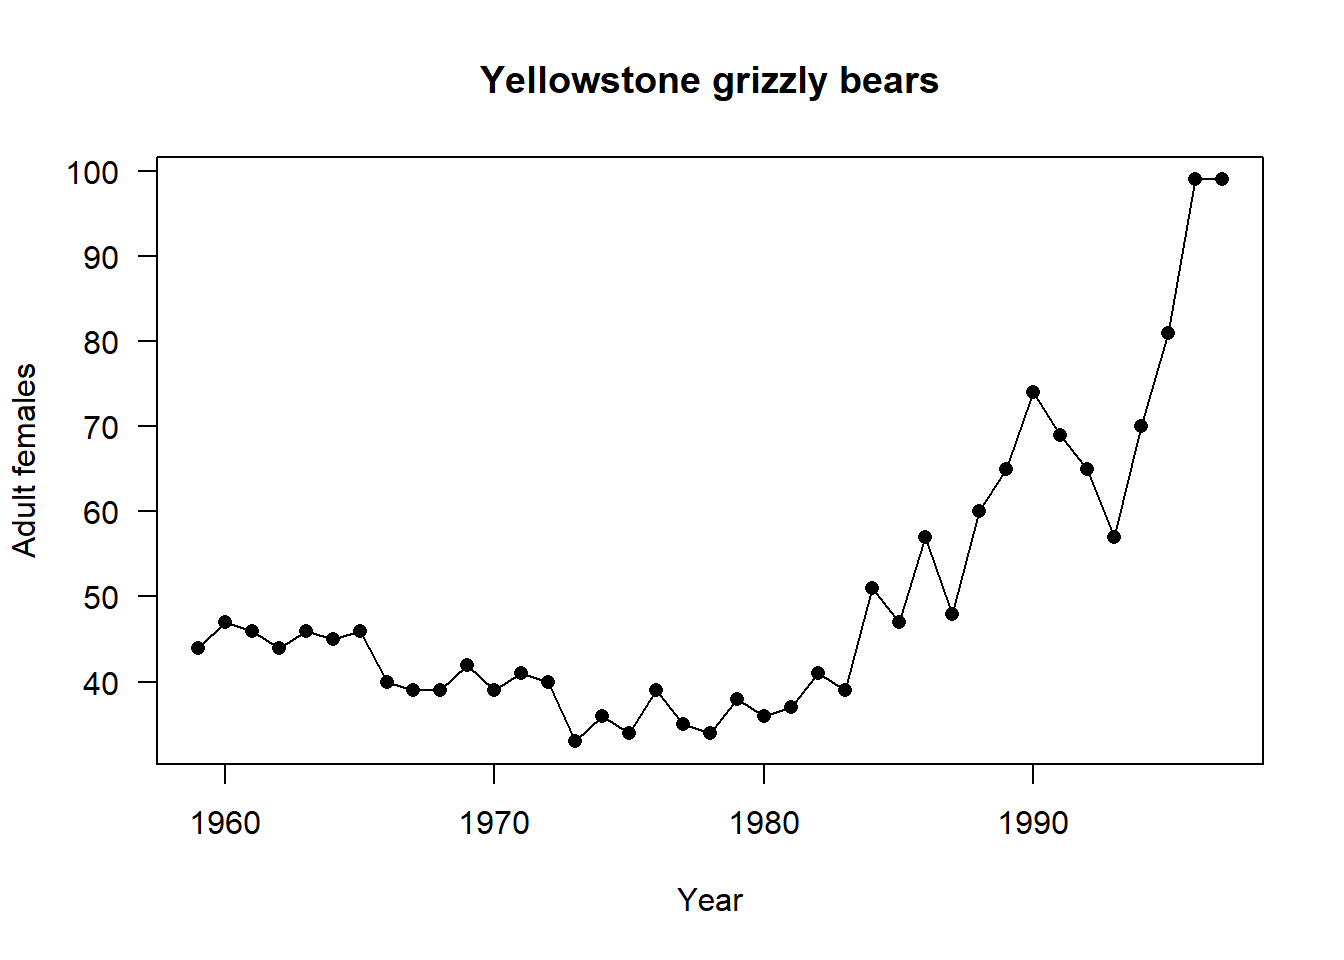
\includegraphics{If_you_go_down_to_the_woods_files/figure-latex/bears-1.pdf}

\hypertarget{what-is-the-grizzly-data-set-all-about}{%
\subsection{What is the grizzly data set all
about}\label{what-is-the-grizzly-data-set-all-about}}

Look up the grizzly dataset from the R help (see above ?grizzly will
search for the dataset in the helpfiles).

Provide a summary of the grizzly dataset

\hypertarget{calculate-the-rate-of-population-change}{%
\subsection{Calculate the rate of population
change}\label{calculate-the-rate-of-population-change}}

Their are only female bears in this count. What could you do to make
this data more representative of the population?

Do we need more data than just female bears?

\hypertarget{use-the-population-models-to-assess-the-population-change-in-bears}{%
\subsection{Use the population models to assess the population change in
bears}\label{use-the-population-models-to-assess-the-population-change-in-bears}}

Make use of only the first 10 years of the bears dataset to predict the
future 17 years. Plot this on the same graph (hint in base R you can add
points to a plot using the ``points()'' fuction)

\#Extra credit:: Make the plots look pretty (look at ?ggplot2 for
example and search on Google for ggplot2)

\begin{Shaded}
\begin{Highlighting}[]
\NormalTok{grizzly[}\DecValTok{1}\OperatorTok{:}\DecValTok{10}\NormalTok{,]}
\end{Highlighting}
\end{Shaded}

\begin{verbatim}
##    year  N
## 1  1959 44
## 2  1960 47
## 3  1961 46
## 4  1962 44
## 5  1963 46
## 6  1964 45
## 7  1965 46
## 8  1966 40
## 9  1967 39
## 10 1968 39
\end{verbatim}

\begin{Shaded}
\begin{Highlighting}[]
\NormalTok{lam<-}\KeywordTok{c}\NormalTok{(}\KeywordTok{rep}\NormalTok{(}\StringTok{"NA"}\NormalTok{,}\DecValTok{9}\NormalTok{))}

\ControlFlowTok{for}\NormalTok{ (i }\ControlFlowTok{in} \DecValTok{2}\OperatorTok{:}\DecValTok{10}\NormalTok{)\{}
\NormalTok{  lam[i]<-grizzly}\OperatorTok{$}\NormalTok{N[i}\OperatorTok{+}\DecValTok{1}\NormalTok{]}\OperatorTok{/}\NormalTok{grizzly}\OperatorTok{$}\NormalTok{N[i]}
\NormalTok{\}}
\NormalTok{lam}
\end{Highlighting}
\end{Shaded}

\begin{verbatim}
##  [1] "NA"                "0.978723404255319" "0.956521739130435"
##  [4] "1.04545454545455"  "0.978260869565217" "1.02222222222222" 
##  [7] "0.869565217391304" "0.975"             "1"                
## [10] "1.07692307692308"
\end{verbatim}

\begin{Shaded}
\begin{Highlighting}[]
\KeywordTok{mean}\NormalTok{(}\KeywordTok{as.numeric}\NormalTok{(lam), }\DataTypeTok{na.rm=}\OtherTok{TRUE}\NormalTok{) }
\end{Highlighting}
\end{Shaded}

\begin{verbatim}
## Warning in mean(as.numeric(lam), na.rm = TRUE): NAs introduced by coercion
\end{verbatim}

\begin{verbatim}
## [1] 0.9891857
\end{verbatim}

\begin{Shaded}
\begin{Highlighting}[]
\KeywordTok{sd}\NormalTok{(}\KeywordTok{as.numeric}\NormalTok{(lam), }\DataTypeTok{na.rm=}\OtherTok{TRUE}\NormalTok{) }
\end{Highlighting}
\end{Shaded}

\begin{verbatim}
## Warning in is.data.frame(x): NAs introduced by coercion
\end{verbatim}

\begin{verbatim}
## [1] 0.05903223
\end{verbatim}

\begin{Shaded}
\begin{Highlighting}[]
\CommentTok{# 0.9891}
\CommentTok{#0.05903223}
\end{Highlighting}
\end{Shaded}

\begin{Shaded}
\begin{Highlighting}[]
\KeywordTok{dim}\NormalTok{(grizzly)}
\end{Highlighting}
\end{Shaded}

\begin{verbatim}
## [1] 39  2
\end{verbatim}

\begin{Shaded}
\begin{Highlighting}[]
\NormalTok{N=}\OtherTok{NULL}

\NormalTok{N[}\DecValTok{1}\NormalTok{]=grizzly}\OperatorTok{$}\NormalTok{N[}\DecValTok{10}\NormalTok{]}

\ControlFlowTok{for}\NormalTok{ (i }\ControlFlowTok{in} \DecValTok{1}\OperatorTok{:}\DecValTok{16}\NormalTok{)\{}
\NormalTok{  N[i}\OperatorTok{+}\DecValTok{1}\NormalTok{]<-}\KeywordTok{rnorm}\NormalTok{(}\DecValTok{1}\NormalTok{,}\FloatTok{0.9891}\NormalTok{, }\FloatTok{0.05903223}\NormalTok{)}\OperatorTok{*}\NormalTok{N[i]}
\NormalTok{\}}

\NormalTok{N}
\end{Highlighting}
\end{Shaded}

\begin{verbatim}
##  [1] 39.00000 39.15690 34.49717 36.39634 35.16374 33.30656 31.42289 31.70242
##  [9] 32.49626 32.16533 26.12769 28.51815 29.54214 28.18735 27.09163 27.02956
## [17] 28.63196
\end{verbatim}

\begin{Shaded}
\begin{Highlighting}[]
\KeywordTok{library}\NormalTok{(tidyverse)}
\end{Highlighting}
\end{Shaded}

\begin{verbatim}
## Warning: package 'tidyverse' was built under R version 4.0.5
\end{verbatim}

\begin{verbatim}
## -- Attaching packages --------------------------------------- tidyverse 1.3.1 --
\end{verbatim}

\begin{verbatim}
## v ggplot2 3.3.5     v purrr   0.3.4
## v tibble  3.1.6     v dplyr   1.0.8
## v tidyr   1.2.0     v stringr 1.4.0
## v readr   2.1.2     v forcats 0.5.1
\end{verbatim}

\begin{verbatim}
## Warning: package 'ggplot2' was built under R version 4.0.5
\end{verbatim}

\begin{verbatim}
## Warning: package 'tibble' was built under R version 4.0.5
\end{verbatim}

\begin{verbatim}
## Warning: package 'tidyr' was built under R version 4.0.5
\end{verbatim}

\begin{verbatim}
## Warning: package 'readr' was built under R version 4.0.5
\end{verbatim}

\begin{verbatim}
## Warning: package 'dplyr' was built under R version 4.0.5
\end{verbatim}

\begin{verbatim}
## -- Conflicts ------------------------------------------ tidyverse_conflicts() --
## x dplyr::filter() masks stats::filter()
## x dplyr::lag()    masks stats::lag()
\end{verbatim}

\begin{Shaded}
\begin{Highlighting}[]
\NormalTok{bears<-}\KeywordTok{data.frame}\NormalTok{(}\DataTypeTok{N=}\NormalTok{N, }\DataTypeTok{years=}\NormalTok{grizzly}\OperatorTok{$}\NormalTok{year[}\DecValTok{10}\OperatorTok{:}\DecValTok{26}\NormalTok{])}
\NormalTok{bears }\OperatorTok\StringTok{ }
\StringTok{  }\KeywordTok{ggplot}\NormalTok{(}\KeywordTok{aes}\NormalTok{(years,N))}\OperatorTok{+}
\StringTok{  }\KeywordTok{geom_point}\NormalTok{(}\DataTypeTok{col=}\StringTok{"blue"}\NormalTok{)}\OperatorTok{+}
\StringTok{  }\KeywordTok{geom_line}\NormalTok{(}\DataTypeTok{col=}\StringTok{"blue"}\NormalTok{)}\OperatorTok{+}
\StringTok{  }\KeywordTok{geom_point}\NormalTok{(}\DataTypeTok{data=}\NormalTok{grizzly, }\KeywordTok{aes}\NormalTok{(year, N), }\DataTypeTok{colour=}\StringTok{"brown"}\NormalTok{)}\OperatorTok{+}
\StringTok{  }\KeywordTok{geom_line}\NormalTok{(}\DataTypeTok{data=}\NormalTok{grizzly, }\KeywordTok{aes}\NormalTok{(year, N), }\DataTypeTok{colour=}\StringTok{"brown"}\NormalTok{)}\OperatorTok{+}
\StringTok{  }\NormalTok{ggthemes}\OperatorTok{::}\KeywordTok{theme_base}\NormalTok{()}
\end{Highlighting}
\end{Shaded}

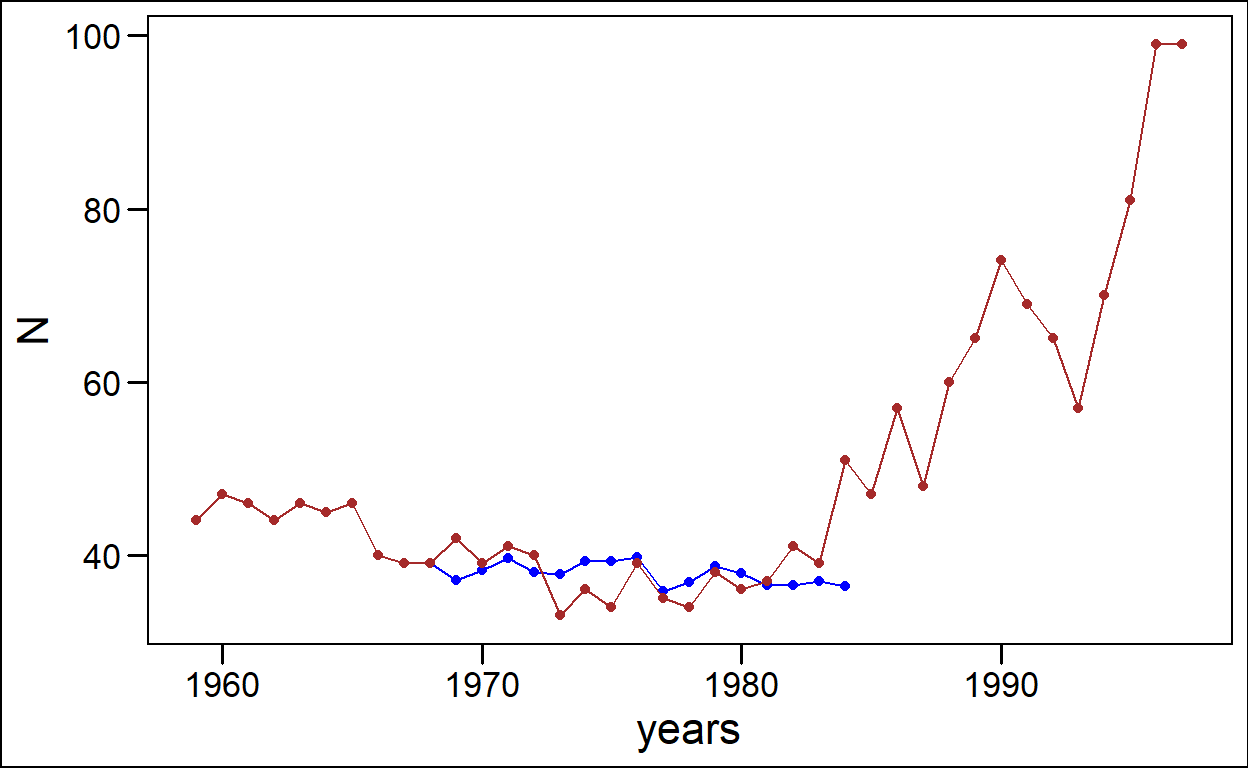
\includegraphics{If_you_go_down_to_the_woods_files/figure-latex/unnamed-chunk-4-1.pdf}

\begin{Shaded}
\begin{Highlighting}[]
\KeywordTok{detach}\NormalTok{(grizzly)}\CommentTok{# remember to detach the data from the session}
\KeywordTok{rm}\NormalTok{(}\DataTypeTok{list=}\KeywordTok{ls}\NormalTok{())}\CommentTok{# this cleans your environment - is useful but }
\CommentTok{#you might want to keep it sometimes - use caution}
\end{Highlighting}
\end{Shaded}

<!--radix_placeholder_site_after_body-->
<!--/radix_placeholder_site_after_body-->

<!--radix_placeholder_navigation_after_body-->
<!--/radix_placeholder_navigation_after_body-->

\end{document}
